%% Software Manual and Technical Document Template	
%% 									
%% This provides an example of a software manual created in Overleaf.

\documentclass{ol-softwaremanual}

% Packages used in this example
\usepackage{graphicx}  % for including images
\usepackage{microtype} % for typographical enhancements
% \usepackage{minted}    % for code listings
\usepackage{amsmath}   % for equations and mathematics
\usepackage{hyperref}  % for hyperlinks
\usepackage{glossaries}
% \setminted{style=friendly,fontsize=\small}
% \renewcommand{\listoflistingscaption}{List of Code Listings}
\usepackage[a4paper,top=4.2cm,bottom=4.2cm,left=3.5cm,right=3.5cm]{geometry}
\usepackage{menukeys}
\usepackage{authblk}
\usepackage{pdfsync}
\usepackage{boldline}
\usepackage{longtable}
\usepackage[version=3]{acro}
\usepackage{gensymb}
% \usepackage[printonlyused,withpage]{acronym}
\usepackage[numbers,sort&compress]{natbib}
\usepackage{anysize}
% \marginsize{2cm}{2cm}{1.cm}               {1.cm}
\usepackage{epsfig}
\usepackage{verbatim} 
\usepackage{bm}
\usepackage{etoolbox}
%\usepackage{amssymb}
%\usepackage{amsfonts,amsmath}
\usepackage{multirow}
% \usepackage[T1]{fontenc}
\usepackage{yfonts}
\usepackage{xr-hyper} 
% \externaldocument{manuscript}
\usepackage{xcite} 
% \externalcitedocument{manuscript}
\usepackage{mathrsfs}
% \usepackage{fancyhdr}
% \usepackage{relsize}
%  \usepackage{newpxtext,newpxmath}
%  \usepackage{booktabs,siunitx}
\usepackage{array,booktabs,ragged2e}
\usepackage{enumitem}   
\usepackage{empheq}
\usepackage[font=small,labelfont=bf]{caption}
\usepackage[title,toc,titletoc,page]{appendix}
\usepackage[capitalise]{cleveref}
\usepackage[most]{tcolorbox}
\usepackage{tocloft}
\usepackage{eurosym}
\usepackage{wrapfig}

\definecolor{glossary-link-color}{RGB}{8,24,168}
\renewcommand*{\glstextformat}[1]{\textcolor{glossary-link-color}{#1}}
\makenoidxglossaries% use TeX to sort

\acsetup{
  make-links ,
  pages / display = first ,
  pages / fill    = {, }
}

\hypersetup{colorlinks=true,
	linkcolor=blue,
	anchorcolor=blue,
	citecolor=red,
	urlcolor=blue
}

\makeatletter
\newcommand*{\glsplainhyperlink}[2]{%
  \colorlet{currenttext}{.}% store current text color
  \colorlet{currentlink}{\@linkcolor}% store current link color
  \hypersetup{linkcolor=brown}% set link color
  \hyperlink{#1}{#2}%
  \hypersetup{linkcolor=currentlink}% reset to default
}
\let\@glslink\glsplainhyperlink
\makeatother

\makeatletter
\def\setmenukeyswin{\def\tw@mk@os{win}}
\def\setmenukeysmac{\def\tw@mk@os{mac}}
\makeatother

\DeclareAcronym{UTC}{short = UTC, long = Universal Time Coordinated}
\DeclareAcronym{TAI}{short = TAI, long = International Atomic Time}
\DeclareAcronym{nm}{
    short = nm, 
    short-plural-form = {nm},
    long = nautical mile
    }
\DeclareAcronym{km}{
        short = km, 
        short-plural-form = {km},
        long = kilometer
}
\DeclareAcronym{hr}{
        short = h, 
        short-plural-form = {hrs},
        long = hour
}
\DeclareAcronym{min}{
        short = min, 
        short-plural-form = {mins},
        long = minute
}
\DeclareAcronym{sec}{
        short = s, 
        short-plural-form = {s},
        long = second
}
\DeclareAcronym{kt}{
    short = kt, 
    short-plural-form = {kts},
    long = knot
    }
\DeclareAcronym{ft}{
    short = ft, 
    short-plural-form = {ft},
    long = foot,
    long-plural-form = {feet}
    }
\DeclareAcronym{m}{
    short = m, 
    short-plural-form = {m},
    long = meter
    }

\DeclareAcronym{N}{
    short = N, 
    long = North
}
\DeclareAcronym{S}{
    short = N, 
    long = South
}
\DeclareAcronym{E}{
    short = E, 
    long = East
}
\DeclareAcronym{W}{
    short = W, 
    long = West
}
\newglossaryentry{sight}{
    name={sight},
    description={the measurement of the height of a celestial body over the horizon},
    plural={sights},
    }
\newglossaryentry{body}{
    name={body},
    description={a celestial object (a star, a planet or a moon) in the sky},
}
\newglossaryentry{route}{
    name={route},
    description={a trajectory on the surface of the Earth, see \cref{fig-route-types}. \thel supports three types of routes: \glspl{loxodrome}, \glspl{orthodrome} and \glspl{circle-of-equal-altitude}},
}
\newglossaryentry{position}{
    name={position},
    description={a location on the surface of the Earth},
}
\newglossaryentry{fix}{
    name={fix},
    description={the calculation of one's \gls{position}. 
    In an astronomical fix, the \gls{position} is obtained as the crossing of multiple \glspl{circle-of-equal-altitude} which result from sextant \glspl{sight}.
    },
}
\newglossaryentry{loxodrome}{
    name={loxodrome},
    description={a \gls{route} forming a constant angle with its local meridians, shown in \cref{fig-route-types}},
}
\newglossaryentry{orthodrome}{
    name={orthodrome},
    description={a \gls{route} which is part of a great circle, show in \cref{fig-route-types}},
}
\newglossaryentry{circle-of-equal-altitude}{
    name={circle of equal altitude},
    description={a curve on the surface of the Earth from which an observer would see a celestial \gls{body} at a given, constant altitude above the horizon, shown in \cref{fig-route-types}},
    plural={circles of equal altitude},
}
\newglossaryentry{transported}{
    name={transported},
    description={a \gls{circle-of-equal-altitude} which comes from a past \gls{sight} is transported long a \gls{route} when its whole route is moved along the \gls{route}'s trajectory. The transporting \gls{route} can be the \gls{route} sailed by the ship in a given time lapse.},
}
\providecommand{\thel}{Thelemacus\,\,}


% Frontmatter data; appears on title page
\title{Documentation}


\version{1.0}
\author{Michele Castellana}
\date{\today\\

\includegraphics[height=0.2\textwidth]{figures/qr-code-thelemacus.png}
\hspace{\stretch{2}} 
\includegraphics[height=0.2\textwidth]{figures/logo-cnrs.png}
}
\softwarelogo{
\includegraphics[width=0.8\textwidth]{figures/title.png}}
\begin{document}
\setlength\intextsep{0pt}


\maketitle

\tableofcontents
\newpage

\section{Introduction}


\thel  is a navigational-astronomy application, which allows to compute one's \gls{position} on the surface of the Earth, on both land and sea, based on \gls{sextant} measurements. 


\subsection{Why \thel?}

Compared to the existing navigational-astronomy softwares, \thel requires the user to enter a smaller amount of data in order to determine his/her \gls{position}; the assumed \gls{position} is not needed. Not only this reduces the chances of making errors, but it also increases the accuracy of the result. 

Also, \thel is conceived to make the user's life easy, and it is designed for an intuitive and ergonomic   use.

\subsection{\thel license}\label{sec-license}

\thel has its own license and  is ``free software''; this means that everyone is free to use it. \thel is not in the public domain \cite{castellana2024thelemacus}; it is copyrighted and there are conditions on its distribution. These conditions are designed to permit everything that a good cooperating citizen would want to do.



\subsection{Obtaining \thel}

The source code for the library can be obtained from its  GitHub \href{https://github.com/mcastel1/thelemacus}{repository}. The executable can be downloaded from my \href{\thelemacusurl}{website}, for both OSx and Windows.  Announcements of new releases, updates and other  events are made \href{\thelemacusurl}{online}. 

\subsection{No warranty}

The \thel has no warranty, use it at your own risk. It is your responsibility to validate the behavior of \thel and its accuracy. 

\thel's provider makes no representations about the
suitability, use, or performance of \thel, or about any
content or information made accessible by it, for any
purpose. \thel is provided ``as is,'' without express or
implied warranties including, but not limited to, any implied
warranties of merchantability, fitness for a particular purpose, or
noninfringement with respect to the software. \thel's provider is not
obligated to support or issue updates to the software.

\subsection{Reporting bugs}

While \thel has now reached a stable, working version, please recall that it is likely to have bugs, and that this is natural. 

A list of known bugs can be found in the \href{\issuesurl}{issues} section of the GitHub repository.
If you find a bug which is not listed in there, please report it to \href{mailto:michele.castellana@gmail.com}{me}. All bug reports should include:
\begin{itemize}
    \item The version number of \thel, 
    \item The hardware and operating system which you used, 
    \item A short description of the bug behavior. 

\end{itemize}

Any errors or omissions in this manual can also be reported to the same address.

\subsection{Improving \thel}

If you have any suggestions to improve \thel or some additional features which you would like to request, please \href{\contactemail}{email me}. 

\subsection{Further information}


Additional information, including online copies of this manual, links to related projects, and mailing list archives are available from \thel \href{\thelemacusurl}{website}  .
Any questions about the use and installation of \thel can be asked by \href{\contactemail}{email}. This mailing address can be used to ask questions not covered by this manual, and to contact \thel developers.

If you would like to refer to \thel in a journal article, the recommended way is to cite this reference manual \cite{castellana2024thelemacus-documentation}. If you want to give a url, use  \href{\thelemacusurl}{this one}. 

\pagebreak

Note that in this manual, if you click on words displayed in {\color{glossary-link-color} this color}, you will be directed to their definition. 

\section{\thel for the impatient}\label{sec-impatient}

\begin{figure}
  \centering
  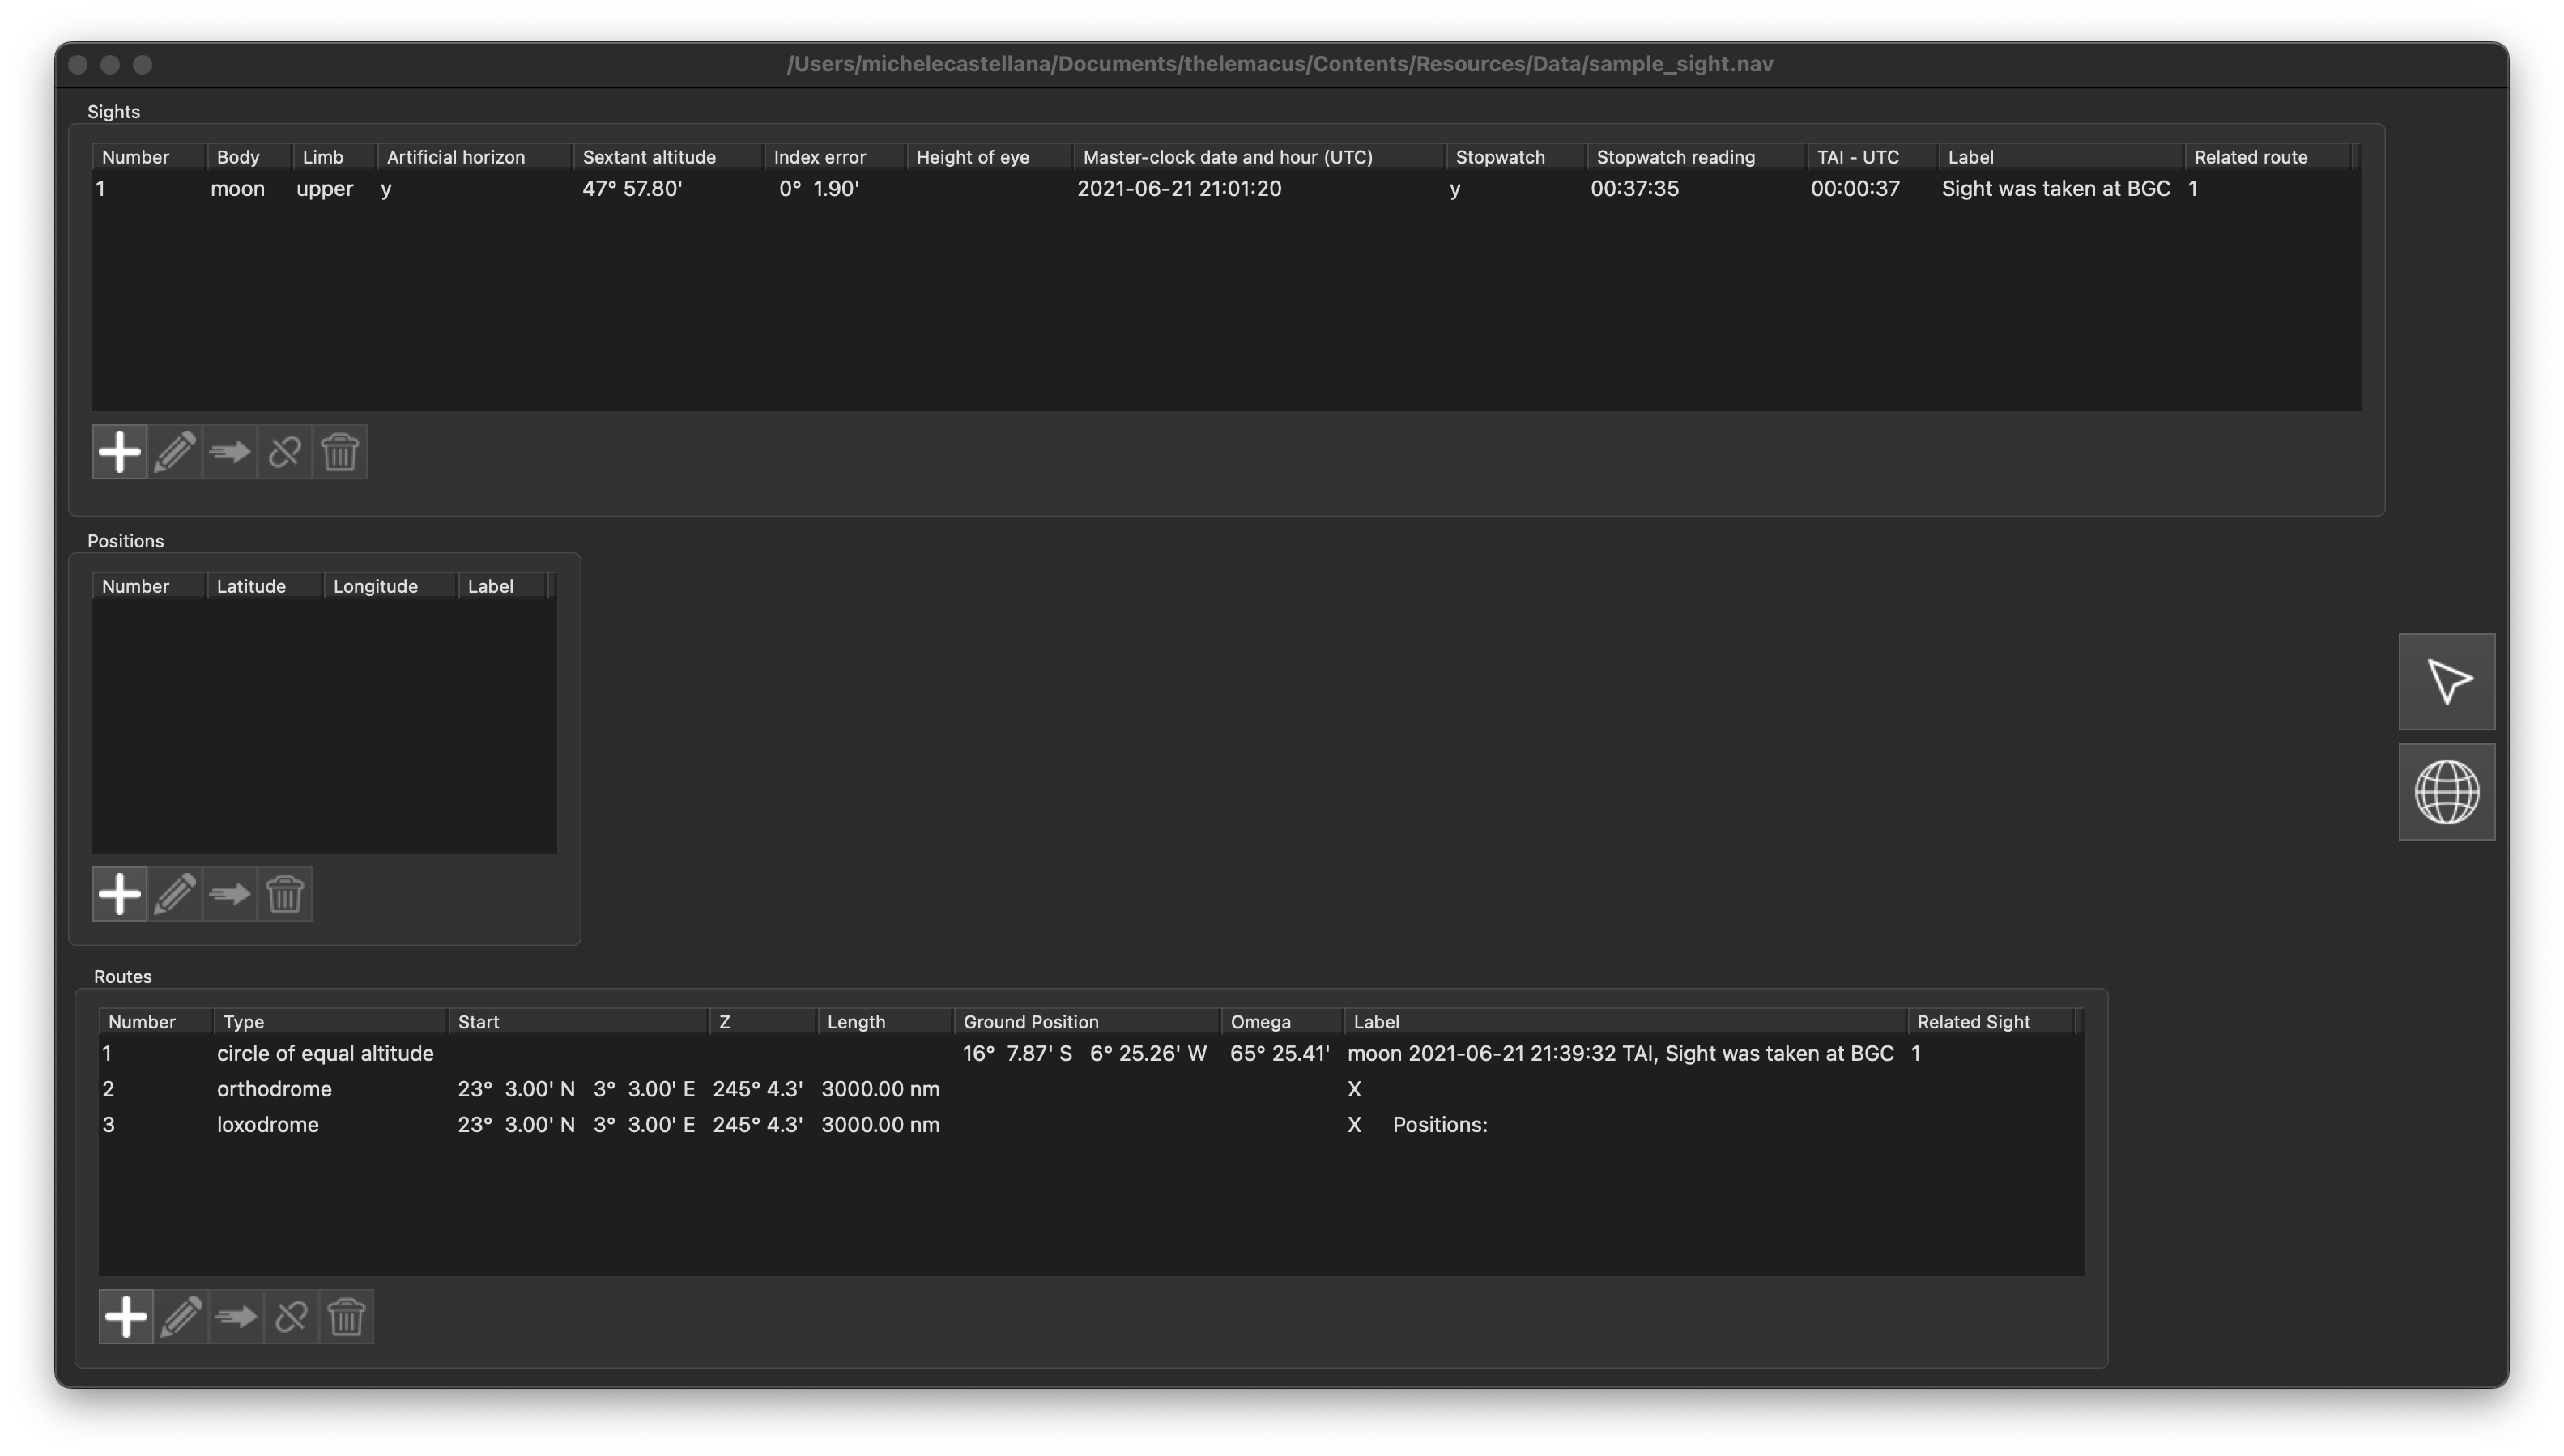
\includegraphics[width=1\textwidth]{figures/list-frame.png}
  \caption{
    \label{fig-list-frame}
    The main frame, where  \gls{sight} and the related \gls{circle-of-equal-altitude} are highlighted in blue.  
  }
  \end{figure}

  \begin{figure}
    \centering
    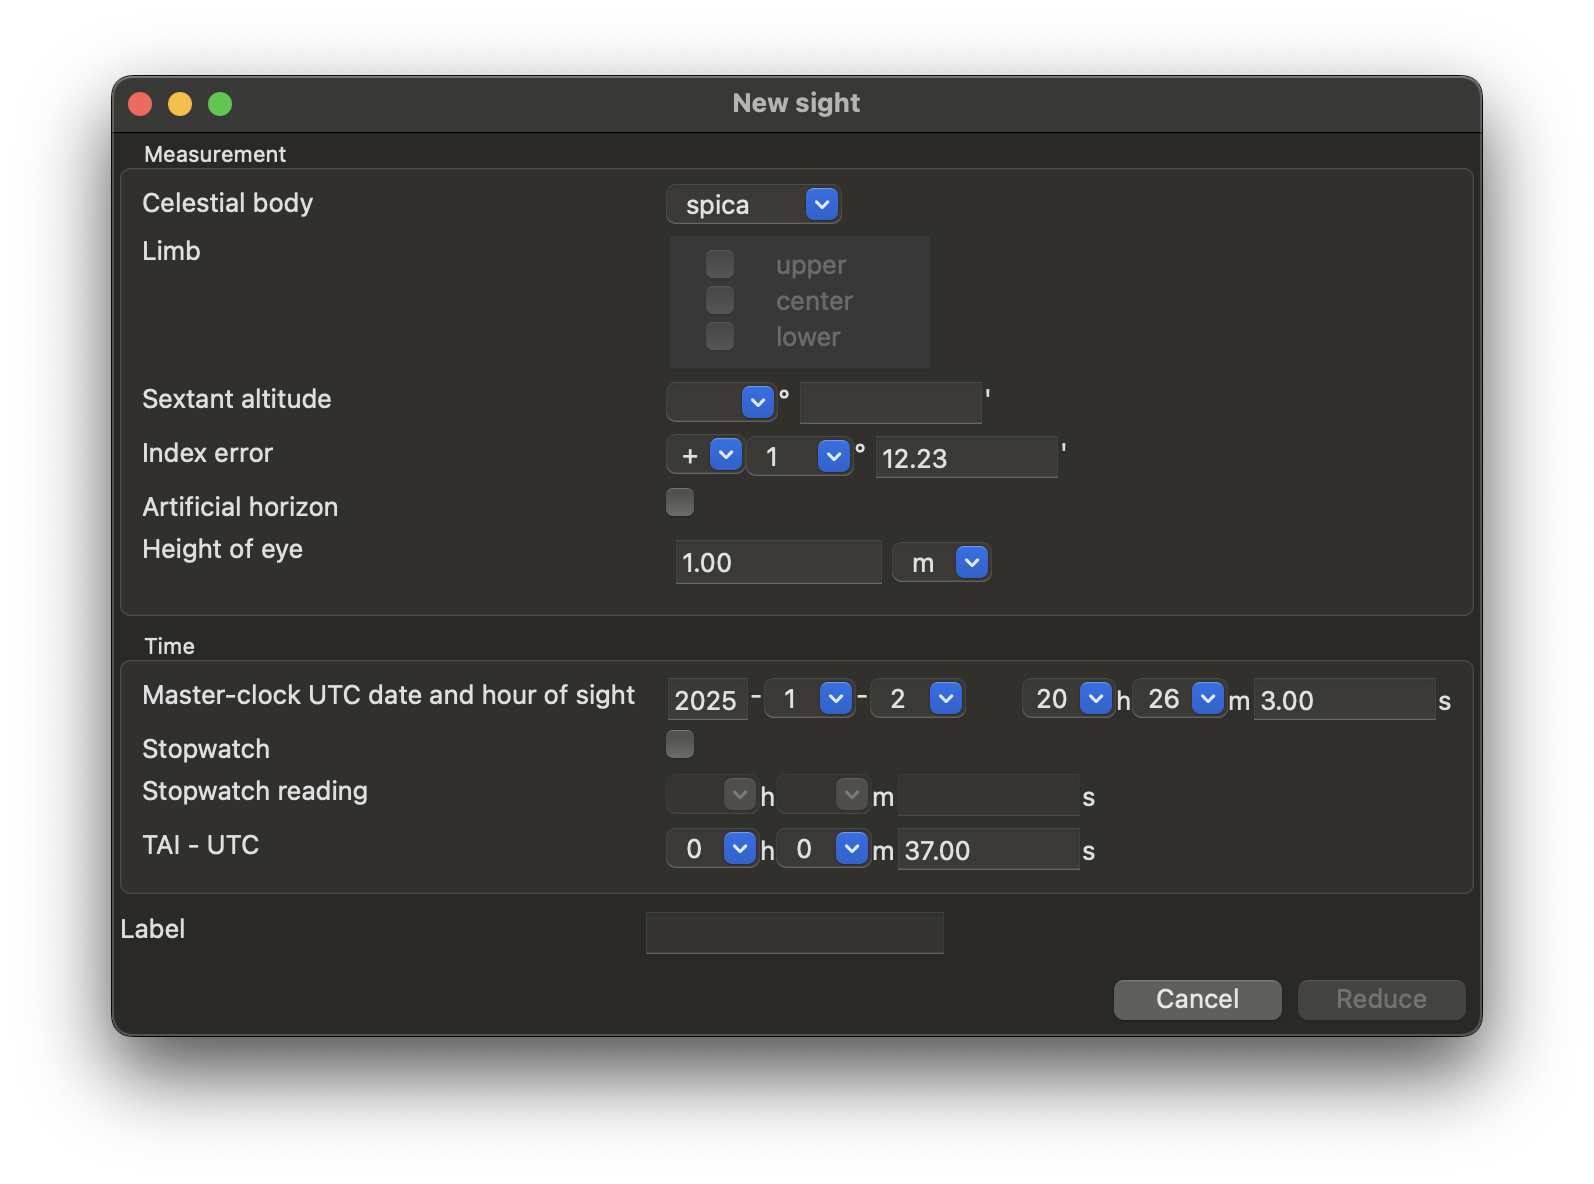
\includegraphics[width=0.9\textwidth]{figures/sight-frame.png}
    \caption{
      \label{fig-sight-frame}
      The \gls{sight} frame with the entered data from \cref{item-name,item-limb,item-body-height,item-artificial-horizon,item-time,item-label,item-index-error,item-observer-height,item-tai-utc,item-stopwatch,item-tai-utc}. 
    }
  \end{figure}

For a quick use of \thel the user may enter a \gls{sextant} \gls{sight}---the measurement of the height of a celestial body over the horizon, with which he/she must be familiar---by going on the main frame of \cref{fig-list-frame} an clicking on \inlinefigure{1.3}{figures/plus-button.png}. A \gls{sight} frame will appear, see \cref{fig-sight-frame}, where the user will enter
\begin{enumerate}
  \item \label{item-name} The name of the celestial \gls{body}, e.g. the star `\href{https://fr.wikipedia.org/wiki/Arcturus}{Arcturus}.' \thel supports the following celestial bodies: Altair, Alpheratz, Arcturus, Capella, Jupiter, Hamal, Kochab, the Moon, Saturn, Sirius, Spica, the Sun and Vega. Other bodies will be added the future. 
  \item \label{item-limb}  If the \gls{body} is the Sun or the Moon, the  limb (`upper', `center' or `lower') of the \gls{body} which has been considered in the measurement (yes/no).
  \item \label{item-body-height} The angular height of the  \gls{body} over the horizon, expressed in degrees and arcminutes,e.g., \myangle{54}{45.34}.
  \item \label{item-artificial-horizon} Whether the observer used an artificial horizon or not for the measurement.
  \item \label{item-time} \ac{UTC} date and time of the measurement, e.g.,
  November 4 2024, $23$ \ac{hr}  $04$ \acp{min} $11$ \acp{sec} \ac{UTC}, which we will write as 
  \mydate{2024}{11}{04} \chrono{23}{4}{11} \ac{UTC}.
  \item \label{item-label} A label to identify the \gls{sight} (optional), e.g., `First \gls{sight} of my night shift.' If no label is entered, \thel will automatically enter as a label the time at which the \gls{sight} was entered. 
  \end{enumerate}
  
  Additional information which, most likely, will have to be modified only once in a while, is: 
  \begin{enumerate}[resume]
    \item \label{item-index-error} The index error \cite{bowditch2002the} of the \gls{sextant}---an angle expressed in degrees and arcminutes, it can be positive or negative---e.g., \myangle{-0}{1.2}.
    \item \label{item-observer-height} The height of the observer above sea level, e.g. $32.3$ \acp{ft}.
    \item \label{item-stopwatch} Whether the observer has used a stopwatch or not and, if so, the stopwatch reading, e.g., \chrono{01}{34}{22}.
    \item \label{item-tai-utc} The difference between \ac{TAI} and \ac{UTC} at the time of the measurement, e.g., \chrono{00}{00}{37}.  You can find the up-to-date value  \href{https://en.wikipedia.org/wiki/Leap_second}{here}. 
  \end{enumerate}

  \begin{figure}
    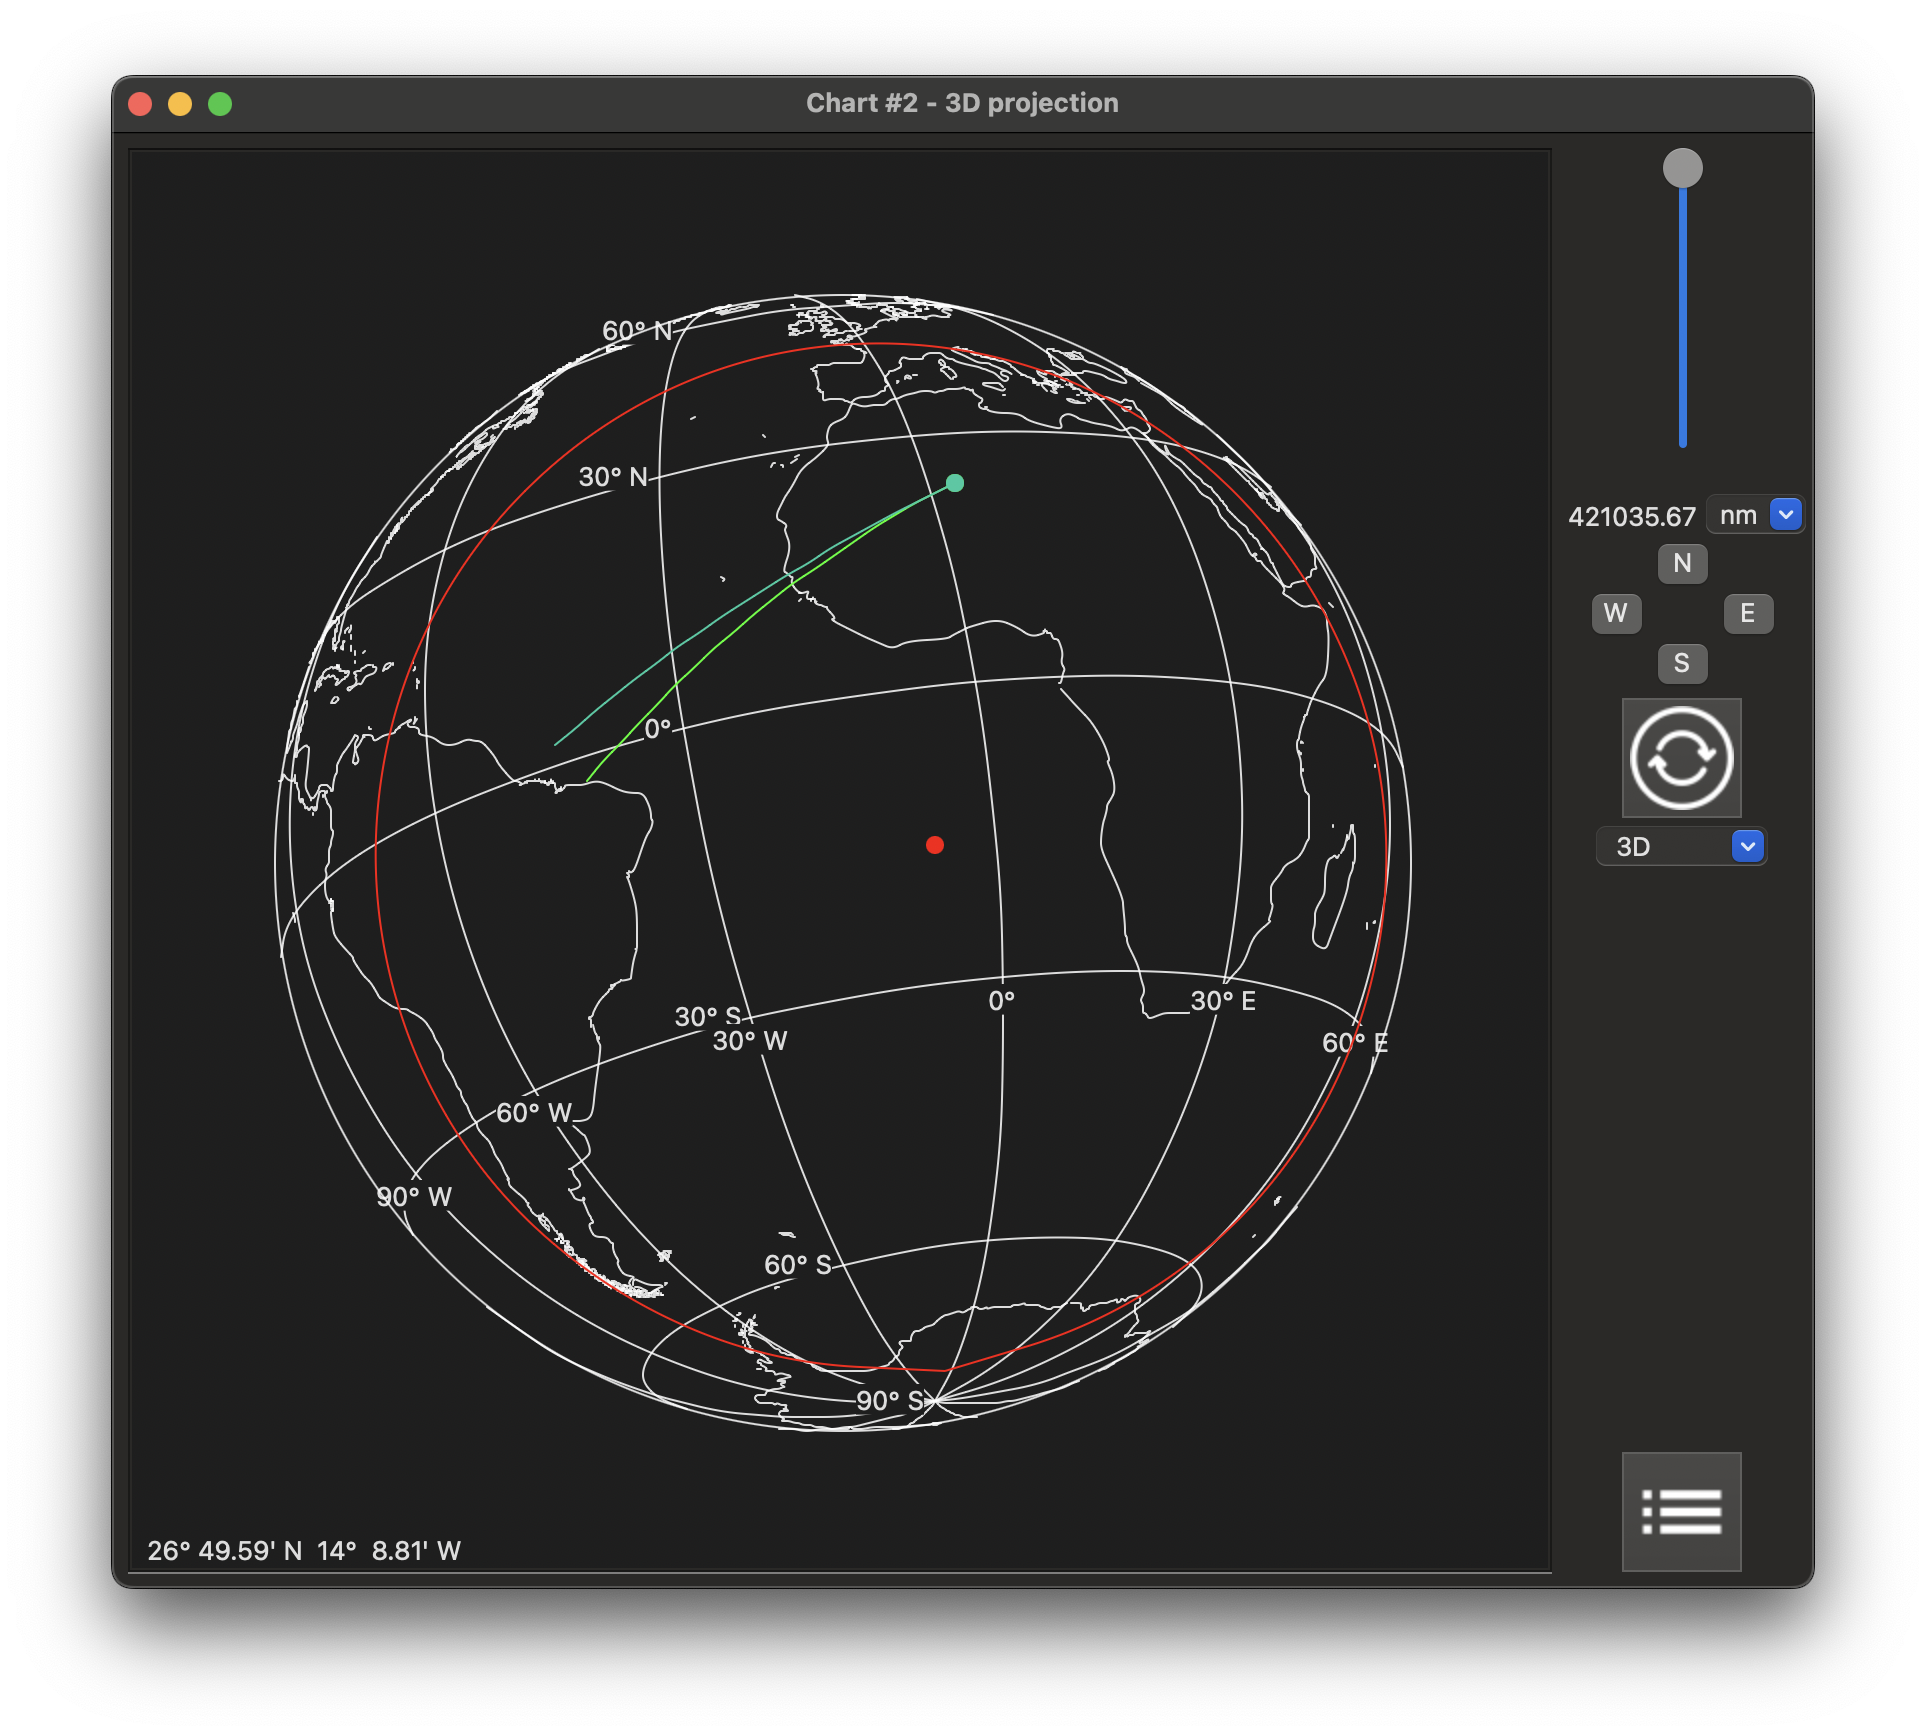
\includegraphics[width=0.6\textwidth]{figures/route-types.png}
    \centering
    \caption{
      \label{fig-route-types}
      The chart frame in the 3d projection showing different \gls{route} types: A \gls{loxodrome} and an \gls{orthodrome} with the same starting point (blue and green, respectively), and a \gls{circle-of-equal-altitude} (red), see \cref{item-route-type}. 
    }
    \end{figure}

  Then click on \inlinefigure{1.3}{figures/button-reduce.png}: \thel will highlight for the user a curve on the surface of the Earth; the user is located somewhere on that curve. 

To compute one's \gls{position}, repeat the procedure above with another \gls{sextant} \gls{sight}, click on the button in \cref{fig-position-button} in the main frame, and select \inlinefigure{1.4}{figures/button-all-routes.png}: \thel will show on the chart the \gls{position}, and list its coordinates in the `\Glspl{position}' box in the main frame. 




\acresetall


\section{\thel complete documentation}



In order to use the full potential of \thel, we encourage the user to get familiar with the following simple concepts, see \cite{bowditch2002the} for details. 

\subsection{Basic concepts}

\subsubsection{\Glspl{sight}} \label{section-sights} 

A \gls{sight} is a measurement of the angular altitude of a celestial \gls{body}, made with a \gls{sextant}. 
The results of this measurements are given in  \cref{item-name,item-limb,item-body-height,item-artificial-horizon,item-time,item-label,item-index-error,item-observer-height,item-tai-utc,item-stopwatch,item-tai-utc}. 



\subsubsection{\Glspl{position}}  \label{section-positions} 

A \gls{position} a  location on the surface of the Earth, specified by 
\begin{itemize}
\item latitude and longitude, e.g., \latlon{54}{45.34}{\ac{N}}, \latlon{156}{42.04}{\ac{E}},
\item a label (optional).
\end{itemize}
\subsubsection{\Glspl{route}} \label{section-routes} 

A \gls{route} is a trajectory, or a curve, on the surface of the Earth, specified by 
\begin{enumerate}
  \item \label{item-route-type} The \gls{route} type , see \cref{fig-route-types}, which can be \cite{bowditch2002the}
  \begin{enumerate}
  \item a \gls{loxodrome}: a curve forming a constant angle with the meridians,
  \item an \gls{orthodrome}: a curve given by a part of a great circle,
  \item  a \gls{circle-of-equal-altitude}: a circle on the surface of the Earth from which an observer would see a celestial \gls{body} at a given, constant altitude above the horizon,
  \end{enumerate}
  \item \label{item-route-azimuth} The \gls{azimuth} $Z$, i.e., the angle between the \gls{route}  and the local meridian at the \gls{route} starting \gls{position}, e.g., \myangle{234}{03.35}.
  \item \label{item-route-length} The length, e.g., the length of the \gls{route} sailed, which can be specified in two ways:
  \begin{enumerate}
  \item by providing the time and speed of the ship, e.g.  \chrono{01}{23}{32} and $5$ \acp{kt}, from which  \thel will extract the length sailed. Speeds can be entered in different units: \acp{kt}, \acp{km}/\ac{hr},  and \acp{m}/\ac{sec}. 
  
  This option is handy when reading off speed and sailed time  on the navigational instruments. 
  \item by providing directly the length sailed by the ship, e.g.,  $15$ \acp{nm}. 
  \end{enumerate}

  \item \label{item-route-reference-position} The start \gls{position} (for \glspl{loxodrome} and \glspl{orthodrome}) or the ground position (for \glspl{circle-of-equal-altitude}), see \cref{section-positions},
  \item \label{item-route-aperture} For \glspl{circle-of-equal-altitude} the aperture angle `omega',
  \item \label{item-route-label} A label (optional). 
\end{enumerate}

\begin{wrapfigure}[10]{R}{0.2\textwidth}
  \centering
  
\includegraphics[width=0.2\textwidth]{figures/position-button.png}
  \caption{\label{fig-position-button} The button to compute the astronomical position.}
  \end{wrapfigure}

When the observer takes a \gls{sight}, then we can conclude that he/she lies on a \gls{route}---a \gls{circle-of-equal-altitude}---on the Earth's surface \cite{bowditch2002the}. 
\textit{Reducing} a \gls{sight} means computing this \gls{route} given the \gls{sight} data in \cref{item-route-reference-position}: we will say that this \gls{route} is \textit{connected} to the \gls{sight}. Importantly, not all \glspl{route} are connected to \glspl{sight}: for example, a \gls{route} denoting the ship's path, or a \gls{circle-of-equal-altitude} originally connected to a \gls{sight} which has been later \gls{transported}, are not. 



\subsection{The main frame}

\thel main frame is shown in \cref{fig-list-frame}, in dark mode.
In this regard, we recall that on macOS \thel switches to light or dark mode automatically, according to the mode of the operating system, while on Windows only light mode is available. 



It is composed of three boxes: 
\begin{enumerate}
  \item \label{item-sight-box} \Gls{sight} box: a table which contains the list of \glspl{sight}---\gls{sextant} measurements of the altitude of a celestial \gls{body} over the horizon. 
  
  Each line in the table corresponds to a \gls{sight}, and its columns are given by: The \gls{sight} identifier, which is automatically assigned by \thel,  the data in \cref{item-name,item-limb,item-body-height,item-artificial-horizon,item-time,item-label,item-index-error,item-observer-height,item-tai-utc,item-stopwatch,item-tai-utc}, and the identifier if the \gls{route} related to the \gls{sight}, see \cref{item-route-box}. 

  To enter a new \gls{sight}, press the \inlinefigure{1.3}{figures/plus-button.png} button at the bottom of the box. To modify or delete an existing \gls{sight}, press  \inlinefigure{1.4}{figures/modify-button.png} or \inlinefigure{1.5}{figures/delete-button.png}, respectively. To transport a \gls{sight}, press \inlinefigure{1.3}{figures/transport-button.png}. 
   To disconnect a \gls{sight} from its \gls{route}, press  \inlinefigure{1.3}{figures/disconnect-button.png}. 


 

  \item \label{item-position-box} Position box: a table which contains the list of entered \glspl{position}. 
  
  Each line corresponds to a \gls{position}, and its columns are given by: The \gls{position} identifier, automatically assigned by \thel,  latitude, longitude, and eventually a label. 

To add a new \gls{position}, modify, transport or delete it, use the buttons at the bottom of the box. 

  \item \label{item-route-box} Route box: Each line corresponds to a \gls{route}, and its columns are given by: The \gls{route} identifier, automatically assigned by \thel, the data in \cref{item-route-type,item-route-azimuth,item-route-length,item-route-reference-position,item-route-aperture,item-route-label}. 

  To add a new \gls{route}, modify, transport, disconnect it from its \gls{sight} or delete it, use the buttons at the bottom of the box. 

\end{enumerate}





If you hover the mouse over a \gls{sight} in the \gls{sight} box, the \gls{sight} will be highlighted. The \gls{route} to which it is connected, both in in the \gls{route} box and in the chart frame, will be highlighted so the user can see directly to what \gls{route} the \gls{sight} corresponds on the chart. Positions and \glspl{route} are highlighted in the same way. 

\begin{wrapfigure}[8]{R}{0.2\textwidth}
  
\includegraphics[width=0.2\textwidth]{figures/tooltip.png}
  \caption{\label{fig-tooltip} Tooltip on the button to show charts in the main frame.}
\end{wrapfigure}



To compute the astronomical \gls{position}, press the position button in \cref{fig-position-button}, and to jump to the charts, press the button in \cref{fig-tooltip}. 


Each button in \thel is equipped with a tooltip: when the mouse lies above the button, a text describing the button's function pops up, see \cref{fig-tooltip}. 




\subsection{The chart frame}\label{section-chart-frame}

The chart frame visually shows  \glspl{route} and \glspl{position} on the surface of the Earth. 

\begin{wrapfigure}[10]{l}{0.2\textwidth}
  
\includegraphics[width=\linewidth]{figures/reset-button.png}
  \caption{\label{fig-reset-button} Button to reset the chart to its original configuration.}
  \end{wrapfigure}

  The user can select two projections \cite{bowditch2002the}, the Mercator projection (\cref{fig-astronomical-position}) and the 3D projection (\cref{fig-route-types}), which shows the Earth as seen from an observer in space. The altitude of the observer is shown as \inlinefigure{1.3}{figures/altitude-field.png}, where the user can change the units of measure to \acp{m}, \acp{ft} or \acp{nm}. 

  \setlength\parfillskip{0pt}\par\setlength\parfillskip{0pt plus 1fil}

\begin{wrapfigure}[10]{r}{0.2\textwidth}
  
\includegraphics[width=\linewidth]{figures/list-frame-button.png}
  \caption{\label{fig-list-frame-button} Button to switch from the chart frame to the main frame.}
  \end{wrapfigure}
  \noindent

  
  

To reset the chart to the original configurations, press the button in \cref{fig-reset-button}, while to jump to the main frame, press the button in \cref{fig-list-frame-button}. 



The coordinates of the instantaneous mouse \gls{position} are shown on the bottom left corner of the chart frame, as \inlinefigure{1.3}{figures/mouse-position.png}. 




\subsubsection{Zooming into the chart} The user can zoom into the chart by either using the mouse wheel, or by using the scroll bar on the top right of the chart frame. Also, one can zoom in a specific area by right-clicking on the chart, moving the mouse to draw a selection rectangle, and right-clicking again, see \cref{fig-selection-rectangle}. To cancel the drawing of the rectangle, press \setmenukeyswin \keys{\esc}. 

\subsubsection{Moving the chart}




To move the chart to the \ac{N}, \ac{S}, \ac{E} or \ac{W}, respectively, use the buttons in \cref{fig-directional-buttons}, or the keyboard keys \keys{\arrowkeyup}, \keys{\arrowkeydown}, \keys{\arrowkeyright} and \keys{\arrowkeyleft}, respectively.  

\begin{wrapfigure}[8]{R}{0.2\textwidth}
  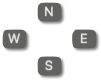
\includegraphics[width=0.2\textwidth]{figures/directional-buttons.png}
  \caption{\label{fig-directional-buttons} Buttons to move the chart \ac{N}, \ac{S}, \ac{E} and \ac{W}. }
  \end{wrapfigure}

\begin{figure}
  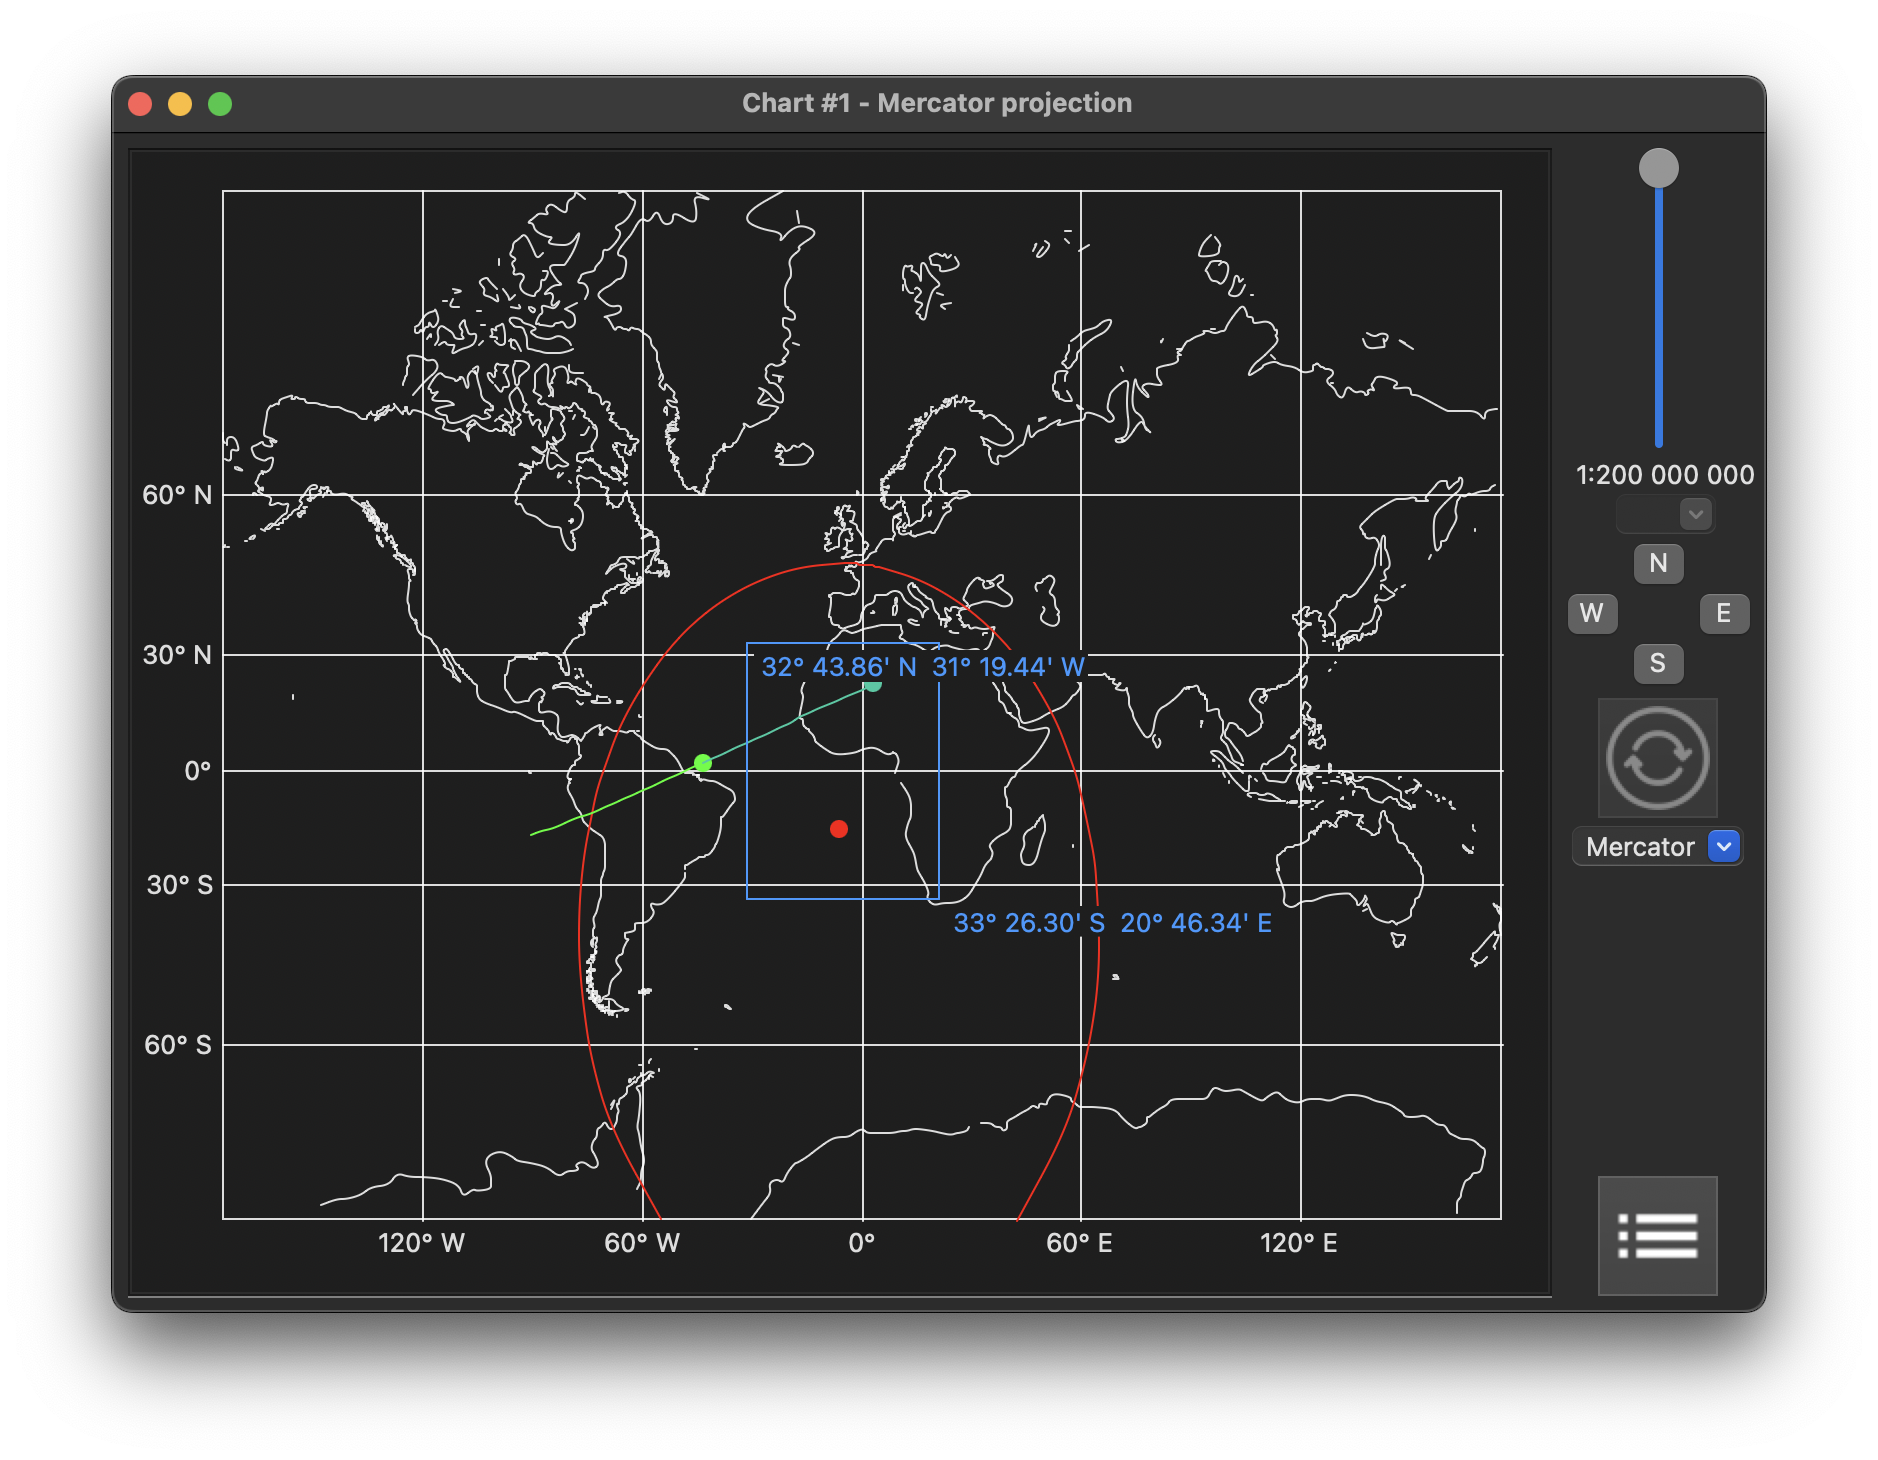
\includegraphics[height=0.4\textwidth]{figures/selection-rectangle-mercator.png}
  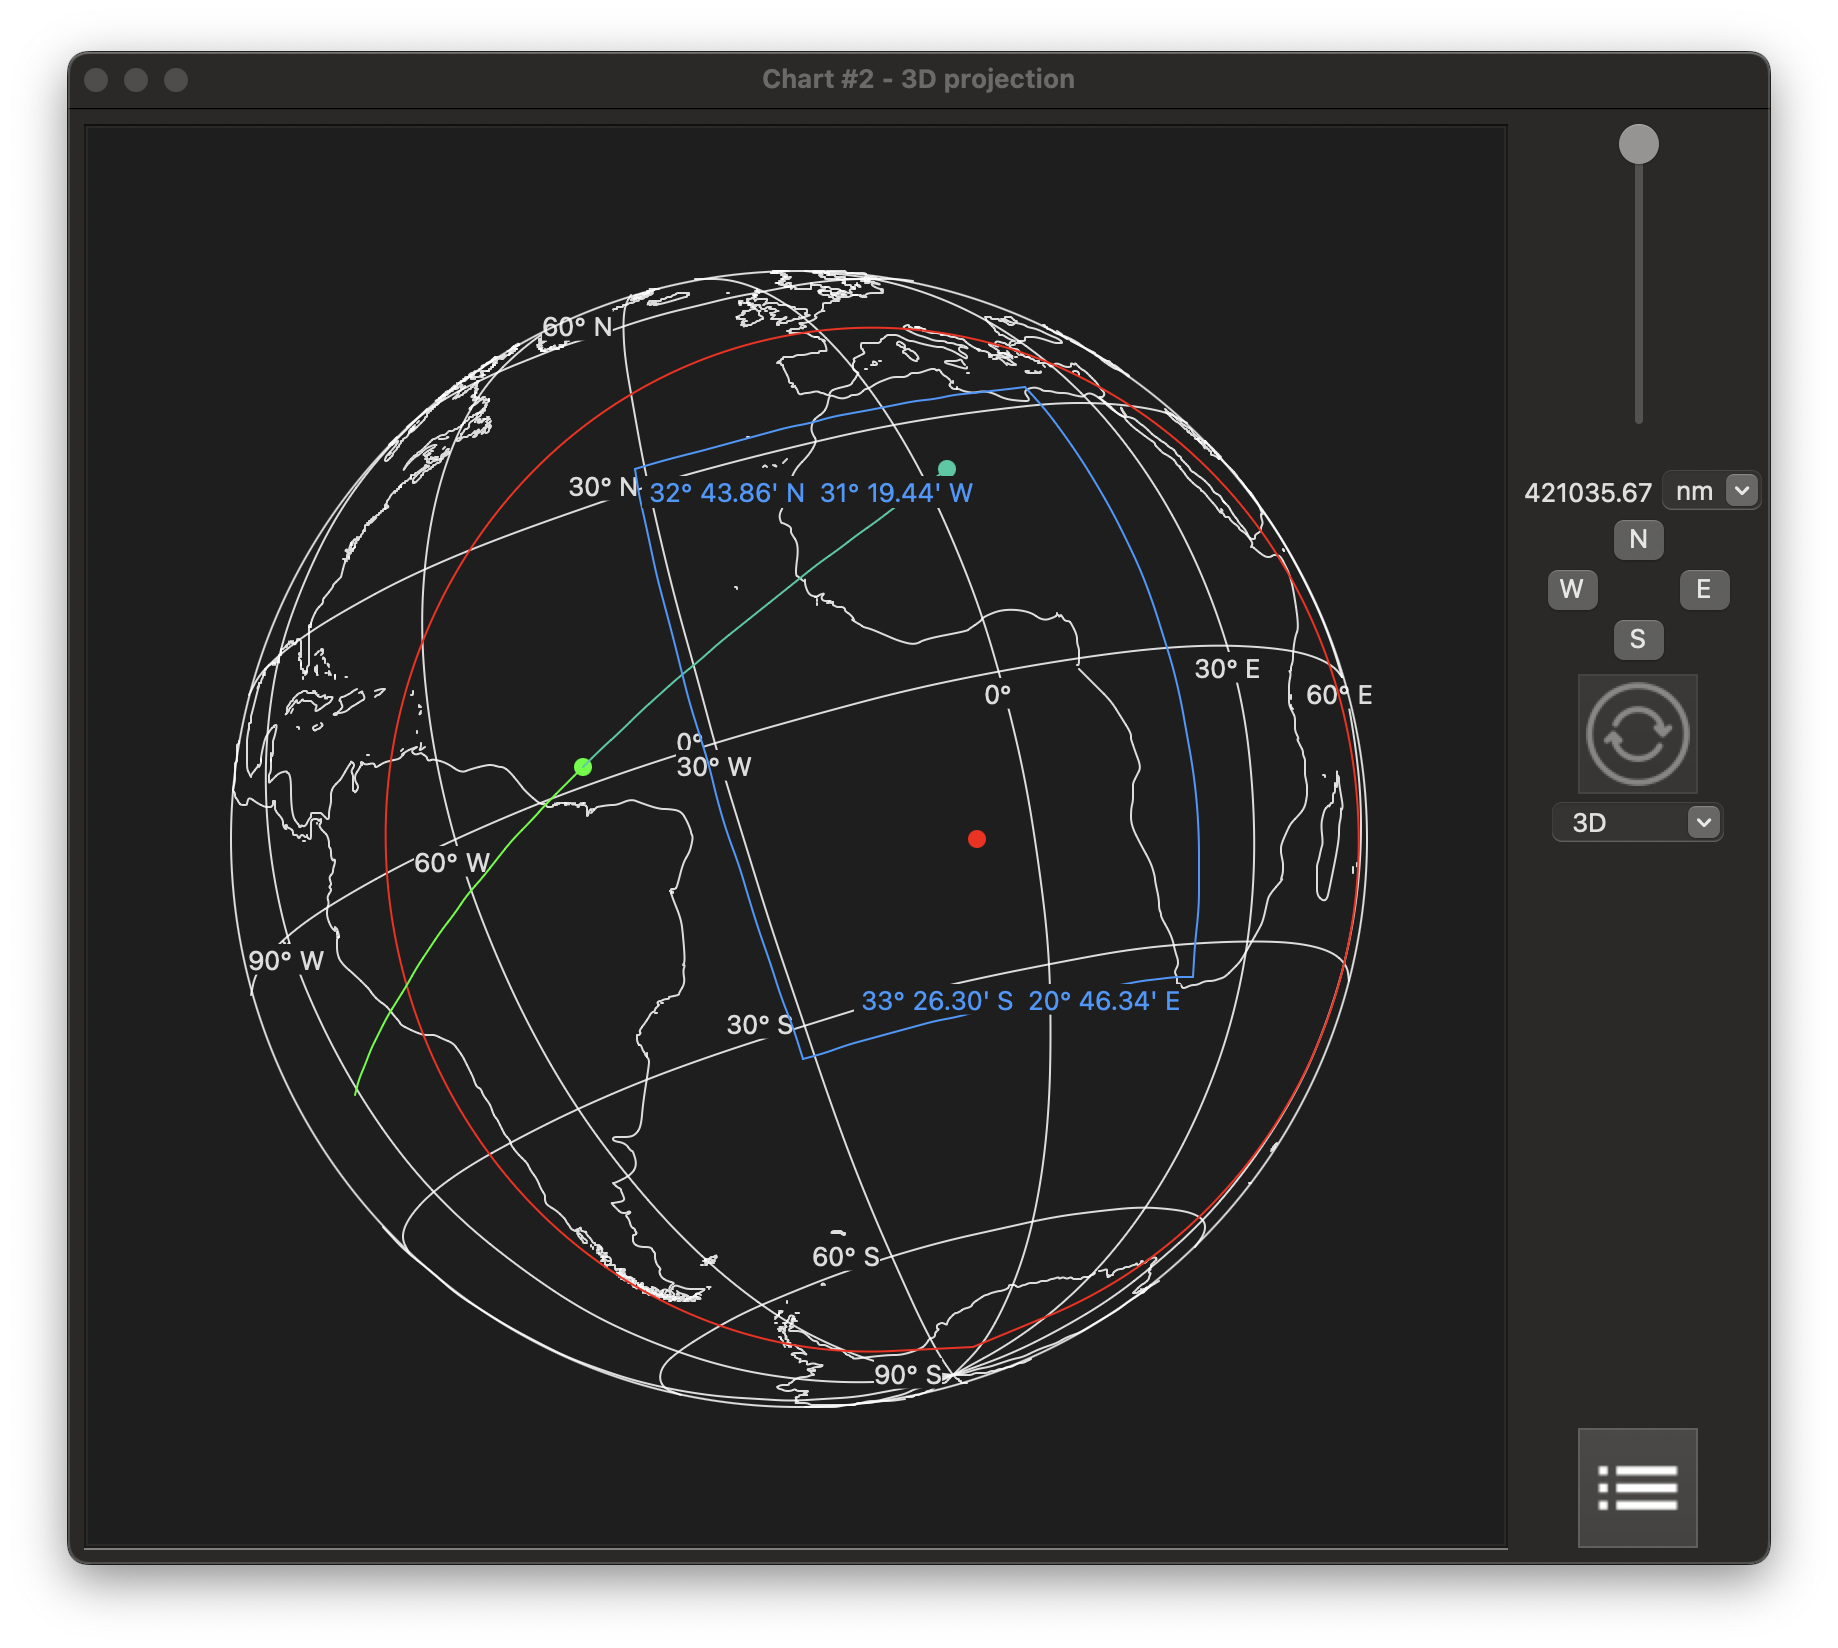
\includegraphics[height=0.4\textwidth]{figures/selection-rectangle-3d.png}
  \caption{
    \label{fig-selection-rectangle}
   The same selection rectangle (blue) shown in the Mercator (left) and in the 3D (right) projection. The coordinates in blue denote the \acl{N}-\ac{W} and \acl{S}-\acl{E} vertices of the rectangle. 
  }
\end{figure}



\subsection{\Glspl{sight}}

\subsubsection{Entering a \gls{sight}: The \gls{sight} frame}

To enter a  \gls{sight}, read  \cref{sec-impatient}  first.  Press  \inlinefigure{1.3}{figures/plus-button.png}, see \cref{fig-list-frame}, a \gls{sight} frame will appear as in \cref{fig-sight-frame}, enter the \gls{sight} fields in  \cref{item-name,item-limb,item-body-height,item-artificial-horizon,item-time,item-label,item-index-error,item-observer-height,item-tai-utc,item-stopwatch,item-tai-utc} of \cref{sec-impatient}, and press \inlinefigure{1.3}{figures/button-reduce.png}.

\textbf{\thel will produce, as output, a \gls{route}}, and trigger a chart animation to it; \textbf{the observer is located  on this route}. This \gls{route} is a \gls{circle-of-equal-altitude}, see \cref{fig-route-types}. 


\begin{figure}
  \centering
  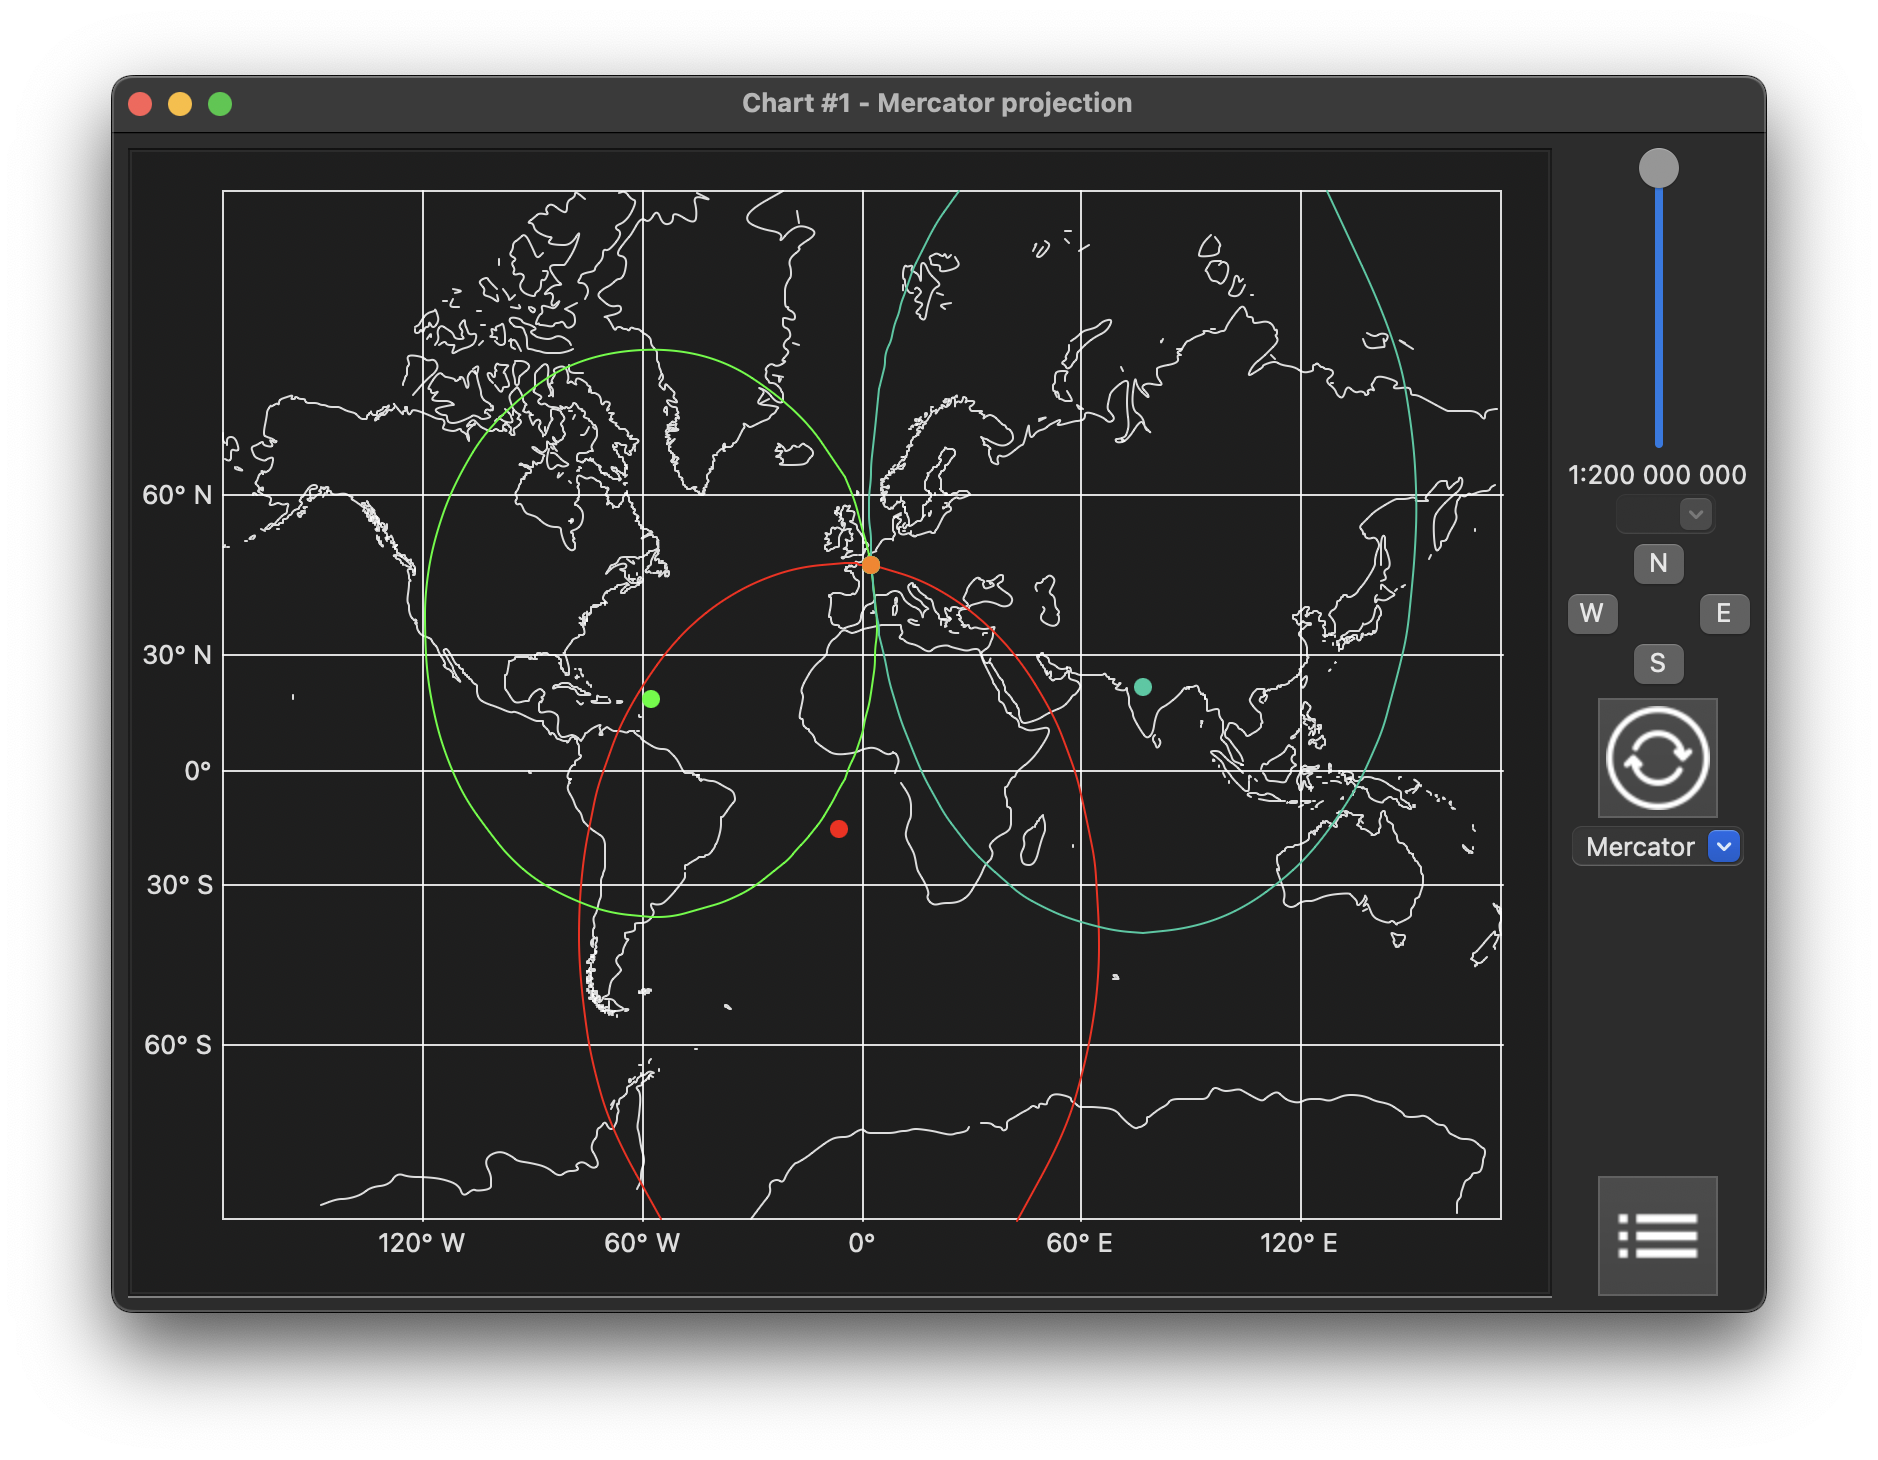
\includegraphics[width=0.9\textwidth]{figures/astronomical-position-mercator.png}
  \caption{
    \label{fig-astronomical-position}
    The chart frame with the Mercator projection, showing the crossing of the three \glspl{route} (red, green and blue) yields the astronomical \gls{position} (orange dot).  
  }
\end{figure}

\subsubsection{Astronomical \gls{fix}}

By making multiple \glspl{sight}, one obtains multiple \glspl{circle-of-equal-altitude}: the astronomical \gls{position} is the crossing point between them---this procedure is called a \gls{fix}. 

To make an astronomical \gls{fix}, click on \inlinefigure{1.3}{figures/position-button.png} in the main frame: the \gls{position} will be added to the \gls{position} list with label `Astronomical \gls{position}', and the charts will display it, see \cref{fig-astronomical-position}. \thel will draw the error on the astronomical \gls{position} as  circle around it, and add it to the \gls{route} list. 




\subsubsection{Transporting a \gls{sight}}\label{section-transporting-sight}

If the course and speed of the ship are known, a \gls{sight} taken in the past can be \gls{transported} and used after it was taken \cite{bowditch2002the,noauthor2017cours}. 

For example, suppose that the observer takes a Sun \gls{sight} (A) in the afternoon, and then a Moon \gls{sight} at dawn (B). \Gls{sight} A can be \gls{transported} along the \gls{route} which the ship sailed between the time of A and that of B. The ship \gls{position} at the time of B is the crossing between A \gls{transported}, and B. 

To transport a sight: 
\begin{itemize}
\item Click on the \gls{sight} in the main frame
\item Click on \inlinefigure{1.3}{figures/transport-button.png} at the bottom of the \gls{sight} box. You can transport the \gls{sight}
\begin{itemize}
\item with a \gls{route} which is already in the \gls{route} box, then press \inlinefigure{1.3}{figures/existing-route-button.png}. Then confirm and select the \gls{route} with which to do the transport by either
\begin{itemize}
  \item double clicking on it, or
  \item selecting it and pressing Enter on the keyboard. 
\end{itemize}
\item with a new \gls{route}: Press \inlinefigure{1.4}{figures/new-route-button.png}, enter the information in the \gls{route} frame, and press \inlinefigure{1.5}{figures/routeframe-transport-button.png}. 
\end{itemize}
\end{itemize}
An animation will move the transporting \gls{route} in place, then transport the \gls{route} related to the \gls{sight}, and move back the transporting \gls{route} to its original \gls{position}. 


\subsection{Positions}\label{section-position}

\begin{figure}
  \centering
  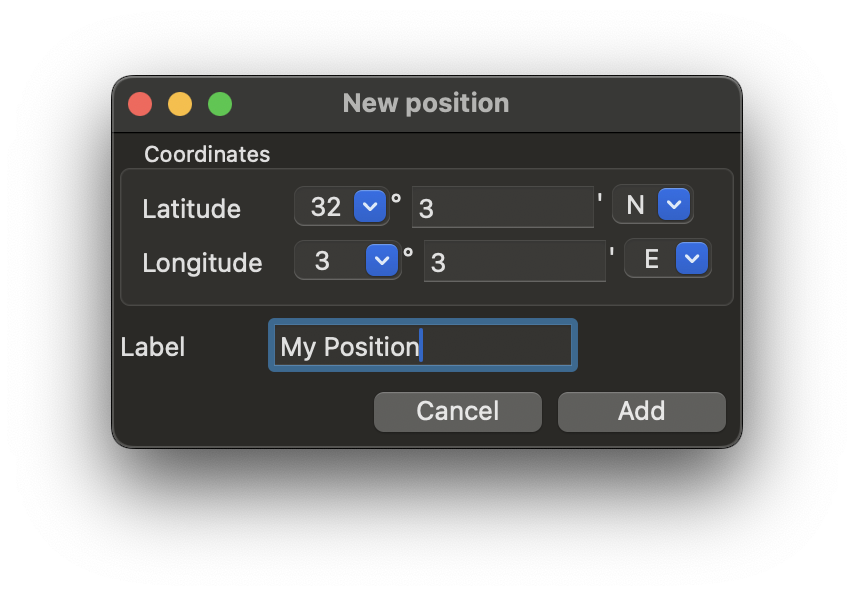
\includegraphics[width=0.4\textwidth]{figures/position-frame.png}
  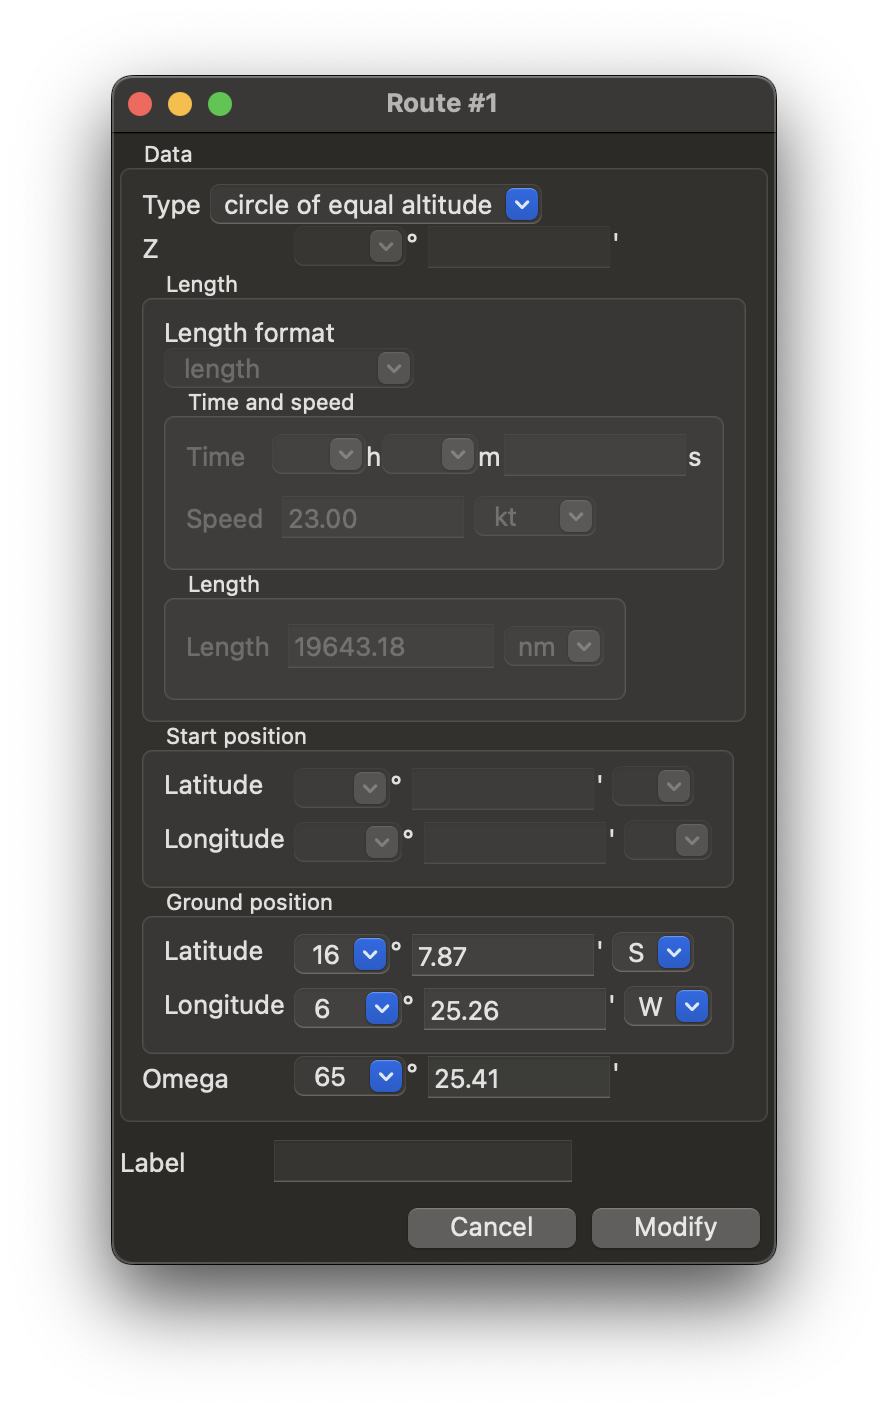
\includegraphics[width=0.4\textwidth]{figures/route-frame.png}
  \caption{
    \label{fig-position-route-frame}
    The \gls{position} frame (left) and the  \gls{route} frame (right).  
  }
\end{figure}


\subsubsection{Entering a \gls{position}}\label{section-enter-position}

To enter a \gls{position}  (for example, the last estimated \gls{position}, or the \gls{position} where something worthwhile happened), go on the main frame and click on \inlinefigure{1.3}{figures/plus-button.png} at the bottom of the \gls{position} frame. The \gls{position} frame will appear, see \cref{fig-position-route-frame}. Fill in the \gls{position} fields of \cref{section-positions} and press \inlinefigure{1.3}{figures/add-button.png}. 

\subsubsection{Transporting a \gls{position}}\label{section-transport-position}

A \gls{position} can be \gls{transported} with a \gls{route} along the lines of a \gls{sight} transport, cf. \cref{section-transporting-sight}. This is useful, for instance, if one needs to transport the a past \gls{fix} according to the recently sailed \gls{route}, in order to obtain the current  \gls{position} \cite{bowditch2002the}. 


\subsection{Routes}\label{section-handle-routes}


\subsubsection{Entering a \gls{route}}\label{section-entering-route}

To enter a \gls{route}, go on the main frame and click on \inlinefigure{1.3}{figures/plus-button.png} at the bottom of the \gls{route} frame. The \gls{route} frame will appear, see \cref{fig-position-route-frame}. Fill in the \gls{route} fields of \cref{section-positions} and press \inlinefigure{1.3}{figures/add-button.png}. 





\subsubsection{Transporting a \gls{route}}\label{section-transporting-route}

A \gls{route} can be \gls{transported} along another \gls{route} just as a  \gls{sight} and \gls{position}, cf. \cref{section-transporting-sight,section-transport-position}. This is useful, for instance, if one needs to transport the a  \gls{circle-of-equal-altitude} of a past \gls{sight} according to the recently sailed \gls{route}, in order to obtain the current \gls{circle-of-equal-altitude} \cite{bowditch2002the}.

\subsection{Loading and saving}\label{sec-load-save}

In \thel, \glspl{sight}, \glspl{position} and \glspl{route} are stored in .nav files. The path of the .nav file where your data is stored is displayed on the top of the main frame, see \cref{fig-list-frame}. 








You can load, save, and `save as' files as by either using \thel menu bar, or the keyboard shortcuts 
\setmenukeysmac
\keys{\cmd + O}, \keys{\cmd + S}, \keys{\cmd + \shift  + S } on OSx, and  
\setmenukeyswin
\keys{\ctrl + O}, \keys{\ctrl + S}, \keys{\ctrl +   \shift + S} on Windows, respectively.  


\pagebreak

\section*{Acknowledgments}

Thanks to Gioia Boschi, Lionel Chiron, Enrico Filippi and Mathieu Coppey for helping me testing \thel and giving useful insights, and Patrick Moreau for his counsel on the software license. 

\printacronyms[pages={display=all,seq/use=false}]

% \printnoidxglossary[style=long]
\printnoidxglossary

\bibliographystyle{unsrt}
%\addcontentsline{toc}{section}{\refname}
\bibliography{/Users/michelecastellana/Documents/my_bibliography/bibliography}


\end{document}
